\documentclass[aspectratio=43]{beamer}
\usepackage[latin1]{inputenc}
\usepackage{amsmath}
\usepackage{amsfonts}
\usepackage{amssymb}
\usepackage{makeidx}
\usepackage{graphicx}
\usepackage{array}
\usepackage{braket}

% Customization
\mode<presentation>{
\usetheme{CambridgeUS}
\usecolortheme{dolphin}
\setbeamertemplate{navigation symbols}{}
}

%\setbeamertemplate{footline}[frame number]

% Title and author
\title[Quantum coherent phenomena]{Quantum coherent phenomena}
\author{\textbf {Jes\'us Urtasun Elizari}}
%\institute{\textbf {University of Milan}}
\date{Milan, October 2020}

\begin{document}

% Front slide
\begin{frame}

	%\maketitle
	\vspace{1.0 cm}
	
	\center{\color{blue}Two-mode squeezed states in cavity optomechanics\\ via engineering of a single reservoir}
	
	\vspace{0.25 cm}
	\center{PhD course - Quantum coherent phenomena\\ Milan, October 2020}

	\begin{figure}
		\minipage{1\textwidth}
		
\includegraphics[width = 3.0 cm]{plots/logo_unimi.png}
		\hfill
		
\includegraphics[width = 3.0 cm]{plots/logo_infn.png}
		\hfill
		
\includegraphics[width = 3.0 cm]{plots/logo_erc.png}
		\endminipage
	\end{figure}

	\vspace{1.0 cm}

\end{frame}

% Introduction
\begin{frame}

	\frametitle{Outline}
	
	\begin{enumerate}
		\item {\color{blue}Introduction, system and Hamiltonian}
		\item {\color{blue}Reservoir engineering strategies}
		\item {\color{blue}Implementation and observable quantities}
		\item {\color{blue}Experimental observability}
		\item {\color{blue}Conclusions}
	\end{enumerate}
	
\end{frame}

% Introduction
\begin{frame}

	\frametitle{Introduction}

	\begin{enumerate}
		\item Generation and detection of entangled states of macroscopic mechanical oscillators
		\item Reservoir engineering $\longrightarrow$ Two-mode squeezed states
		\item Easy to implement in existing experimental configurations
		\item Quantum optomechanics $\longrightarrow$ describe mesoscopic systems
	\end{enumerate}	
	
\end{frame}

% System and Hamiltonian I
\begin{frame}

	\frametitle{Introduction}
	\framesubtitle{System representation}
	
	\begin{itemize}
		\item Two mechanical oscillators with resonance frequencies $\omega_{a}, \omega_{b}$
		\item Dispersively coupled $g_{a}, g_{b}$ to a common cavity $\omega_{c}$
		\item Radiation pressure forces inside the cavity lead motion of the mirrors become highly entangled
	\end{itemize}

		\begin{figure}
			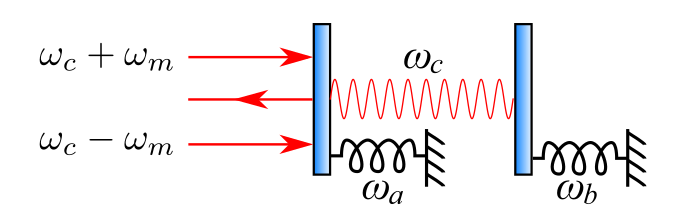
\includegraphics[width = 8 cm]{plots/plot_system.png}
		\end{figure}	

\end{frame}

% System and Hamiltonian II
\begin{frame}
	
	\frametitle{Introduction}
	\framesubtitle{System and Hamiltonian}
	
	Quantum optomechanics $\longrightarrow$ Hamiltonian describing optical and mechanical modes with same formalism 
	\begin{figure}
		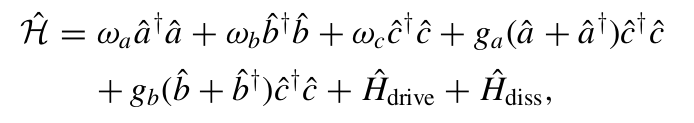
\includegraphics[width = 8 cm]{plots/hamiltonian_1.png}
	\end{figure}
	
	Under usual approximations {\color{blue}}, obtain the master formula 
	\begin{figure}
		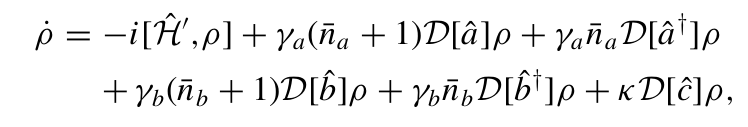
\includegraphics[width = 8 cm]{plots/master_eq_1.png}
	\end{figure}

	Being $\mathcal{H}' = \mathcal{H} - \mathcal{H}_{\textrm{diss}}$, and $\mathcal{D}[\hat{c}]$ the dispersive superoperator\\
	Only dissipation term for $\hat{c} \longrightarrow$ {\color{blue}Assuming cavity is at T = 0}
	
\end{frame}

% Reservoir engineering I
\begin{frame}
	
	\frametitle{Reservoir engineering strategies}
	\framesubtitle{Bogoliubov operators}
	
	Define the {\color{blue}Bogoliuov} mechanical modes in terms of the modes $\hat{a}, \hat{b}$
	\begin{figure}
		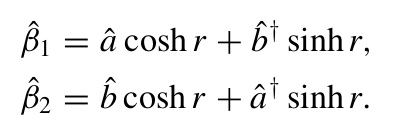
\includegraphics[width = 5 cm]{plots/bogoliubov_1.png}
	\end{figure}	

	being r the {\color{blue}squeezing parameter}\\
	Work in rotating frame with respect to the Hamiltonian
	\begin{figure}
		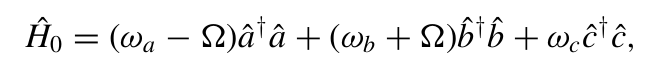
\includegraphics[width = 8 cm]{plots/hamiltonian_2.png}
	\end{figure}	

	where choice of detuning $\Omega$ is such that collective mechanical quadratures $\hat{X}_{\pm}$, $\hat{P}_{\pm}$ rotate in a non-trivial way

\end{frame}

% Reservoir engineering II
\begin{frame}

	\frametitle{Reservoir engineering strategies}
	\framesubtitle{Note on squeezed modes}
	
	Squeezed modes minimize the variance of quadrature operators
	\begin{figure}
		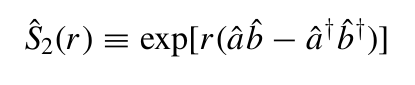
\includegraphics[width = 5 cm]{plots/2_squeezed_mode.png}
	\end{figure}	
	
	\begin{figure}
		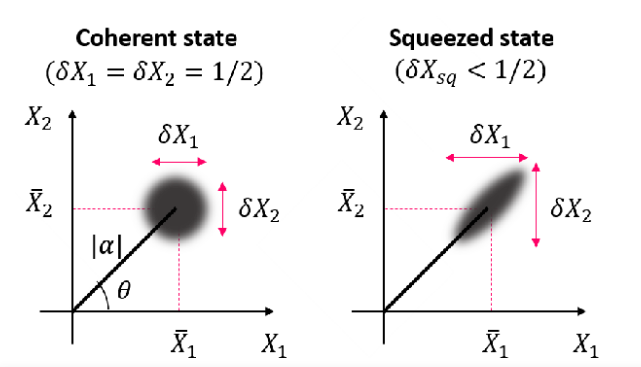
\includegraphics[width = 7 cm]{plots/plot_squeezed.png}
	\end{figure}

\end{frame}

% Reservoir engineering III
\begin{frame}
	
	\frametitle{Reservoir engineering strategies}
	\framesubtitle{2-mode squeezed state}
	
	Define the 2-mode squeezed as $\ket{r}_{2} = \hat{S}_{2}(r) \ket{0,0}$
	\begin{figure}
		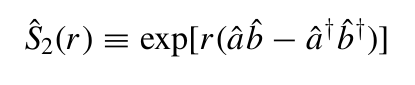
\includegraphics[width = 5 cm]{plots/2_squeezed_mode.png}
	\end{figure}	

	such that $[\hat{S}_{2}(r) \hat{a} \hat{S}_{2}^{\dagger}(r)]\ket{r}_{2} = [\hat{S}_{2}(r) \hat{b} \hat{S}_{2}^{\dagger}(r)]\ket{r}_{2} = 0$\\
	
	\vspace{0.5cm}
	
	Therefore, $\hat{\beta}_{1} = \hat{S}_{2}(r) \hat{a} \hat{S}_{2}^{\dagger}(r)$, $\hat{\beta}_{2} = \hat{S}_{2}(r) \hat{b} \hat{S}_{2}^{\dagger}(r)$ and their\\ground state is the two-mode squeezed state with squeezing parameter $r$

\end{frame}

% Reservoir engineering V
\begin{frame}
	
	\frametitle{Reservoir engineering strategies}
	\framesubtitle{Note on Quantum Optomechanics}
	
	Linearized Hamiltonian with 2-tone laser with amplitudes $\alpha_{\pm}$)
	
	\begin{equation}
	\mathcal{H} = \hbar \textrm{g}_{+} \; (a^{\dagger}b^{\dagger} + ab) + \hbar \textrm{g}_{-} \; (a^{\dagger}b + ab^{\dagger}) \nonumber
	\end{equation}
	
	being $g_{\pm} = g_{0} \alpha_{\pm}$ \\
	Study different cases
	
	\begin{itemize}
		\item $g_{-} = 0 \longrightarrow$ Sideband blue $\mathcal{H} = \hbar \textrm{g} \; (a^{\dagger}b^{\dagger} + ab)$ "2 - mode squeezing"
		\item $g_{+} = 0 \longrightarrow$ Sideband red $\mathcal{H} = \hbar \textrm{g} \; (a^{\dagger}b + ab^{\dagger})$ "beam - splitter"
		\item $g_{-} = g_{+} = g \longrightarrow \mathcal{H} = \hbar \textrm{g} \; (a + a^{\dagger})(b + b^{\dagger})$ "back-action evading"
	\end{itemize}	

\end{frame}

% Reservoir engineering VI
\begin{frame}
	
	\frametitle{Reservoir engineering strategies}
	\framesubtitle{Generate the 2-mode squeezed state}
	
	\begin{itemize}
		\item i) Two cavity modes to independently cool the Bogoliubov modes (beam splitter $\hat{\beta}^{\dagger}_{i} \hat{c}_{i}$)
		\item ii) Couple the cavity to one Bogoliubov mode  ($\hat{\beta}^{\dagger}_{1} \hat{c}$), and then this to the other ($\hat{\beta}^{\dagger}_{1} \hat{\beta}_{2}$)
		\item iii) Couple the cavity to sum of the Bogoliubov modes , then the sum to the difference (beam splitter $\hat{\beta}^{\dagger}_{\textrm{sum}} \hat{\beta}_{\textrm{diff}}$ allows diff to cool).
		\begin{align}
			\hat{\beta}_{\textrm{sum}} = \frac{1}{\sqrt{2}}(\hat{\beta}_{1} + \hat{\beta}_{2}) \nonumber \\
			\hat{\beta}_{\textrm{diff}} = \frac{1}{\sqrt{2}}(\hat{\beta}_{1} - \hat{\beta}_{2}) \nonumber
		\end{align}
	\end{itemize}

	Cooling $\hat{\beta}_{\textrm{sum}}$ and $\hat{\beta}_{\textrm{diff}}$ is equivalent to cool $\hat{\beta}_{1}$ and $\hat{\beta}_{2} \qquad \checkmark$

\end{frame}

% Reservoir engineering VII
\begin{frame}
	
	\frametitle{Reservoir engineering strategies}
	\framesubtitle{Hamiltonian}
	
	Hamiltonian in terms of the Bogoliubov modes
	\begin{figure}
		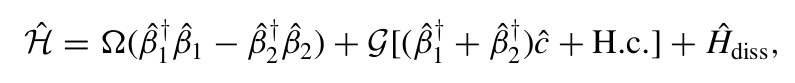
\includegraphics[width = 8.5 cm]{plots/hamiltonian_3.png}
	\end{figure}	
	
	where $\Omega$ is the effective frequency and $\mathcal{G}$ an effective coupling.
	
	Written in terms of the original operators,
	\begin{figure}
		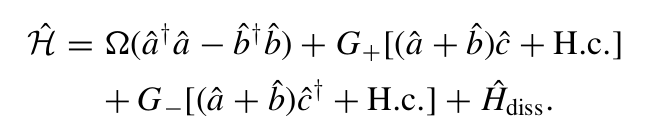
\includegraphics[width = 7.5 cm]{plots/hamiltonian_4.png}
	\end{figure}

	with couplings related by $\mathcal{G} \equiv \sqrt{G_{-}^{2} - G_{+}^{2}}$ and $\tanh r \equiv G_{+}/G_{-}$

\end{frame}

% Implementation I
\begin{frame}

	\frametitle{Implementation}
	\framesubtitle{Different cases}
	
		$\mathcal{H}$ is already implemented in conventional optomechanical setups. Focus on regime $|G_{+}|<|G_{-}|$\\
		Quantum optomechanics Hamiltonian in terms of $\beta_{1}$ and $\beta_{2}$ modes

	\begin{itemize}
		\item Two-tone driving $(g_{a} = g_{b}) \longrightarrow$ cavity drive tones at $\omega_{c} \pm \omega_{m}$ 
		\item Four-tone driving ($g_{a} = g_{b}$)
		\item Case similar ($g_{a} \sim g_{b}$)
	\end{itemize}	

\end{frame}

% Implementation - 2 tone driving
\begin{frame}

	\frametitle{Implementation}
	\framesubtitle{2 - tone driving}
	
	Couplings equal $\longrightarrow$ driving tones $\omega_{c} \pm \omega_{m}$ being  $\omega_{m} = (\omega_{a} + \omega_{b}) / 2$
	
	\begin{figure}
		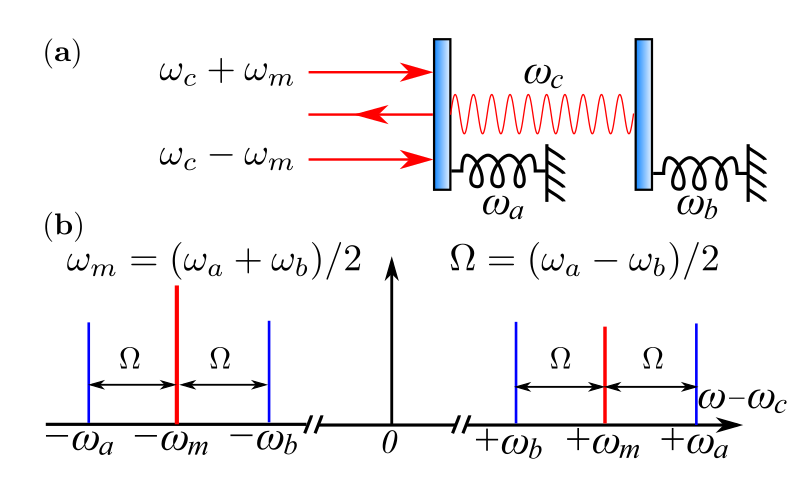
\includegraphics[width = 7 cm]{plots/plot_2_tone.png}
	\end{figure}	

	Apply our drive Hamiltonian

	\begin{figure}
		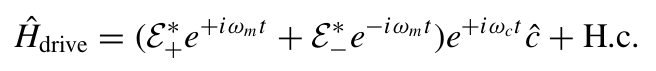
\includegraphics[width = 7 cm]{plots/hamiltonian_2_tone.png}
	\end{figure}

\end{frame}

% Implementation - 2 tone driving
\begin{frame}
	
	\frametitle{Implementation}
	\framesubtitle{2 - tone driving}
	
	Couplings equal $\longrightarrow$ driving tones $\omega_{c} \pm \omega_{m}$ being  $\omega_{m} = (\omega_{a} + \omega_{b}) / 2$
	Driving tones applied with single relative phase\\
	Interaction picture with respect to $\mathcal{H}_{0}$ leads to H (8) $\checkmark$\\
	
	\begin{itemize}
		\item Steady state in terms of the driving frequency, amplitude of the laser and dissipation
		\begin{figure}
			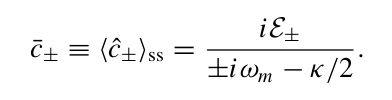
\includegraphics[width = 5 cm]{plots/ss_2_tone.png}
		\end{figure}
		\item Assumptions used (...)
	\end{itemize}

\end{frame}

% Implementation - 4 tone driving
\begin{frame}
	
	\frametitle{Implementation}
	\framesubtitle{4 - tone driving}
	
	Driving tones applied with detuning of $\Omega$ from the sidebands $\omega_{c} \pm (\omega_{a} - \Omega)$ and $\omega_{c} \pm (\omega_{b} + \Omega)$
	
	\begin{figure}
		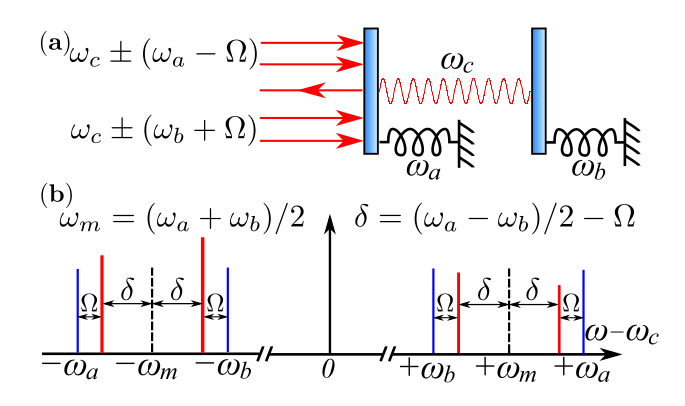
\includegraphics[width = 7 cm]{plots/plot_4_tone.png}
	\end{figure}	
	
	\begin{figure}
		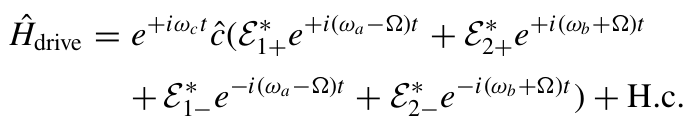
\includegraphics[width = 8 cm]{plots/hamiltonian_4_tone.png}
	\end{figure}

\end{frame}

% Implementation - 4 tone driving
\begin{frame}
	
	\frametitle{Implementation}
	\framesubtitle{4 - tone driving}
	
	Couplings unequal $\longrightarrow$ driving tones applied with detuning of $\Omega$ from the sidebands $\omega_{c} \pm (\omega_{a} - \Omega)$ and $\omega_{c} \pm (\omega_{b} + \Omega)$\\
	Interaction picture with respect to $\mathcal{H}_{0}$ leads to H (14) $\checkmark$
	\begin{figure}
		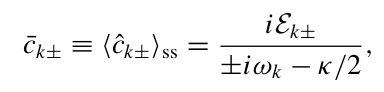
\includegraphics[width = 5 cm]{plots/ss_4_tone.png}
	\end{figure}

	\begin{itemize}
		\item Where we demand the strengths match as $\bar{c}_{1\pm} / \bar{c}_{2\pm} = g_{b} / g_{a}$
		\item Working in interaction picture with respect to Hamiltonian (4)
		\item Imprecision in the matching lead to add contributions as in Hamiltonian (14)
	\end{itemize}

	Condition $\gamma \ll \Omega \ll (\omega_{a} - \omega_{b})/2 - \gamma$, {\color{blue}sufficiently coupled} Bogoliubov modes and unwanted sideband processes have no effect.

\end{frame}

% Adiabatic limit I
\begin{frame}
	
	\frametitle{Adiabatic limit}
	\framesubtitle{Our system}
	
	\begin{itemize}
		\item Assume the system responds rapidly to mechanical motion $k > \Omega, G_{\pm}$, but still in the regime $\omega_{a}, \omega_{b} \gg k$
		\item Simplify by getting rid of the cavity operator $\hat{c} = -2i\mathcal{G}(\hat{\beta}_{1} + \hat{\beta}_{2})/k$\\
		\item Obtain adiabatically eliminated master equation
	\end{itemize}

	\begin{figure}
		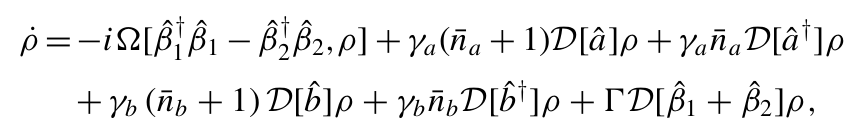
\includegraphics[width = 9 cm]{plots/master_eq_2.png}
	\end{figure}

	with optomechanical damping rate
	\begin{figure}
		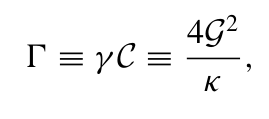
\includegraphics[width = 3 cm]{plots/optomechanic_dumping.png}
	\end{figure}

	Easy to obtain steady state, and to measure entanglement and purity.
	 
\end{frame}

% Adiabatic limit II
\begin{frame}
	
	\frametitle{Adiabatic limit}
	\framesubtitle{Entanglement}
	
	Build a way of identify entanglement on a 2-mode system\\
	Duan criterion $\longrightarrow$ define collective quadratures
	\begin{figure}
		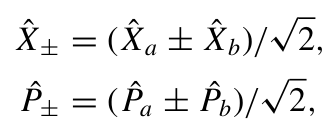
\includegraphics[width = 4 cm]{plots/entanglement_quad.png}
	\end{figure}	
	
	as combination of the usual quadrature modes
	\begin{figure}
		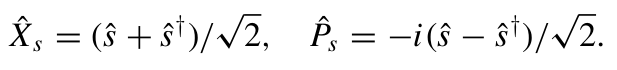
\includegraphics[width = 7 cm]{plots/entanglement_quad_2.png}
	\end{figure}

	Duan inequality states that a state for which
	\begin{figure}
		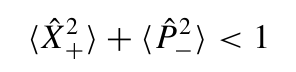
\includegraphics[width = 3.5 cm]{plots/entanglement_duan_criterion.png}
	\end{figure}

	is inseparable.

\end{frame}

% Adiabatic limit III
\begin{frame}

	\frametitle{Adiabatic limit}
	\framesubtitle{Entanglement}
		
	Quadratures can be written as function of the drive asymmetry 
	\begin{figure}
		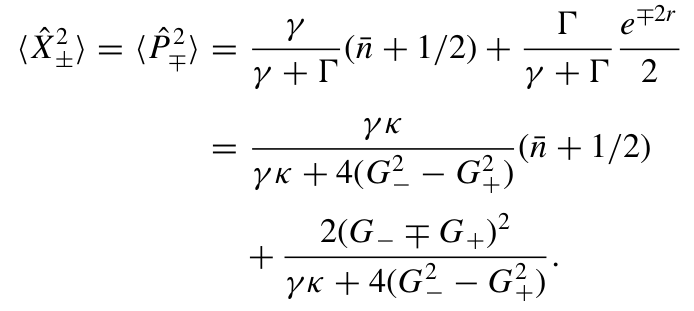
\includegraphics[width = 7.5 cm]{plots/entanglement_quadratures.png}
	\end{figure}

	Use also logarithmic negativity 

\end{frame}

% Adiabatic limit IV
\begin{frame}
	
	\frametitle{Adiabatic limit}
	\framesubtitle{Purity}
	
	Study purity of the steady state\\
	Highly entangled does not imply highly pure\\
	
	Purity defined as trace of the density matrix
	\begin{equation}
		\mu \equiv \textrm{tr}[\rho^{2}] \nonumber
	\end{equation}	
		
	As function of the covariance matrix
	\begin{equation}
		\mu = \frac{1}{4 \sqrt{\det \textbf{V}}} \nonumber
	\end{equation}
	Purity can be written as function of the drive asymmetry 
	\begin{figure}
		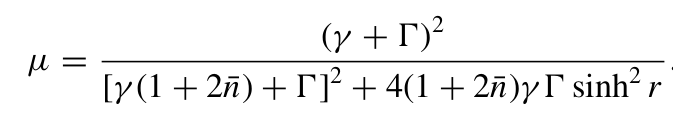
\includegraphics[width = 6.5 cm]{plots/purity.png}
	\end{figure}

\end{frame}

% Adiabatic limit V
\begin{frame}
	
	\frametitle{Adiabatic limit}
	\framesubtitle{Entanglement}
	
	\begin{columns}
		
		\column{0.5\textwidth}
		
		\begin{figure}
			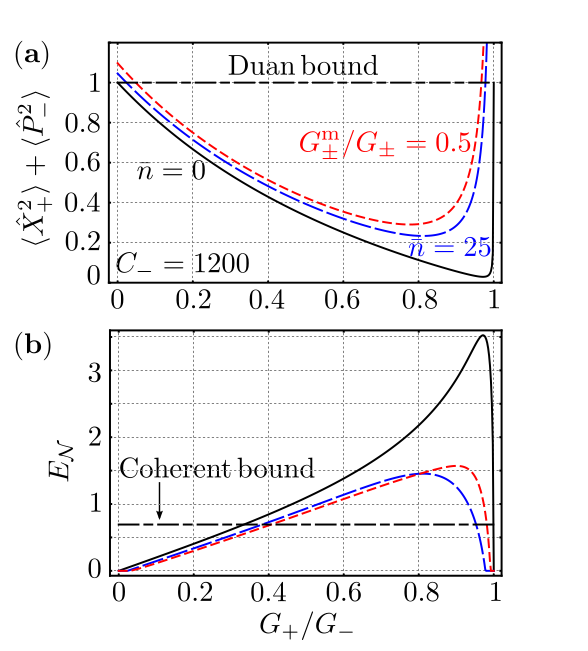
\includegraphics[width = 6 cm]{plots/plot_entanglement.png}
		\end{figure}	
	
		\column{0.65\textwidth}
		
		\begin{itemize}
			\item Case $\gamma_{a} = \gamma_{b}$ and $\bar{n}_{a} = \bar{n}_{b}$
			\item Solid curve with mechanical thermal occupation $\bar{n} = 0$ and no imperfections on effective coupling $G^{m}_{\pm} = 0$
			\item Add thermal occupation leads to less entanglement
			\item Add drive asymmetry leads to less entanglement
		\end{itemize}
		
	\end{columns}

\end{frame}

% Adiabatic limit IV
\begin{frame}
	
	\frametitle{Adiabatic limit}
	\framesubtitle{Entanglement}
	
	\begin{columns}
		
		\column{0.5\textwidth}
		
		\begin{figure}
			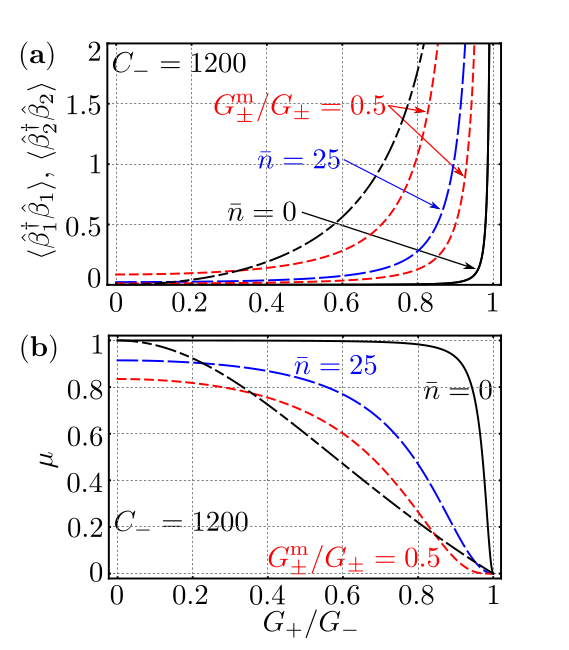
\includegraphics[width = 6 cm]{plots/plot_steady_state.png}
		\end{figure}	
		
		\column{0.65\textwidth}
		
		\begin{itemize}
			\item Solid curve with mechanical thermal occupation $\bar{n} = 0$ and no imperfections on effective coupling $G^{m}_{\pm} = 0$
			\item Add thermal occupation leads to less entanglement
			\item Add drive asymmetry leads to less entanglement
		\end{itemize}
		
	\end{columns}

\end{frame}

% Time dependence
\begin{frame}

\frametitle{Time dependence}
\framesubtitle{Counter rotating terms and time dependence}

	\begin{figure}
		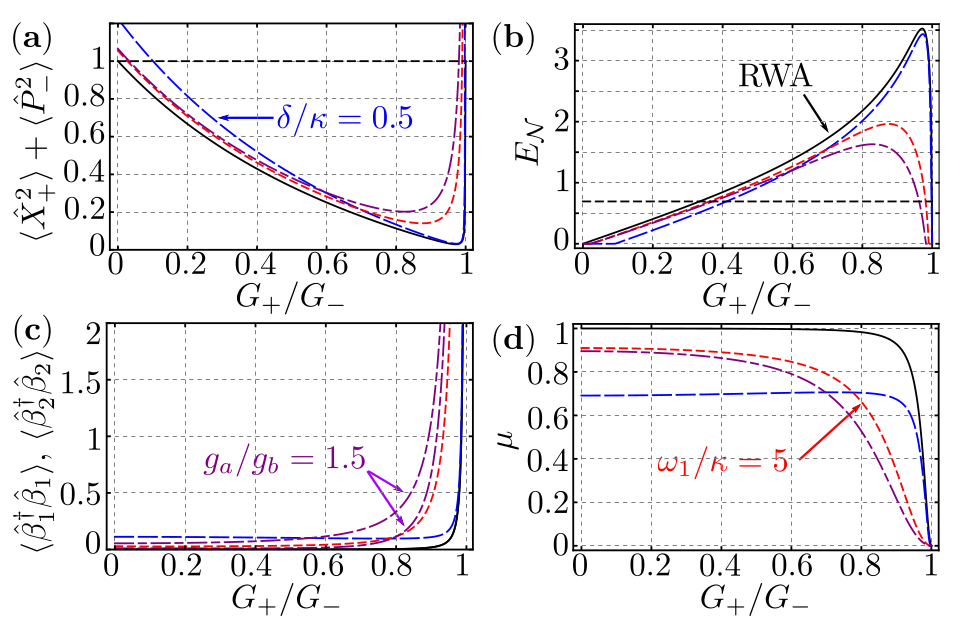
\includegraphics[width = 9 cm]{plots/plot_time_dependence.png}
	\end{figure}	
	
	Counter-rotating effects lead to degradation of entanglement and purity\\
	RWA recovers recovers the behavior of time-independent Hamiltonian
\end{frame}

% Experimental observability
\begin{frame}
	
	\frametitle{Experimental observability}
	\framesubtitle{Output spectrum}
	
	\begin{itemize}
		\item Extremely demanding reconstruct covariance matrix
		\item Directly measure quadratures is a hard problem
		\item Seek signature of entanglement in output spectrum
	\end{itemize}

	Spectrum as Fourier transform of expected value	
	\begin{figure}
		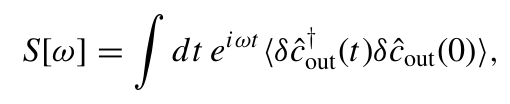
\includegraphics[width = 6 cm]{plots/spectrum_fourier.png}
	\end{figure}	

	being $\delta \hat{c}_{\textrm{out}} = \hat{c}_{\textrm{out}} - <\hat{c}_{\textrm{out}}>$ \\
	Spectrum can be related to the occupation of modes
	\begin{figure}
		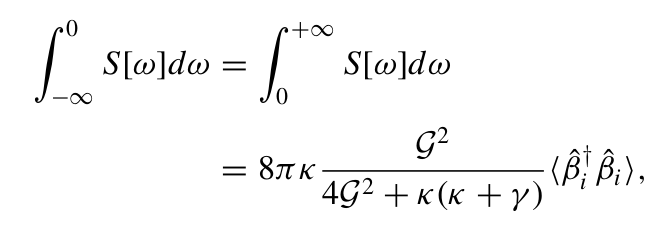
\includegraphics[width = 6.5 cm]{plots/spectrum.png}
	\end{figure}	

\end{frame}

% Experimental observability
\begin{frame}

\frametitle{Experimental observability}
\framesubtitle{Output spectrum}
	
	\begin{figure}
		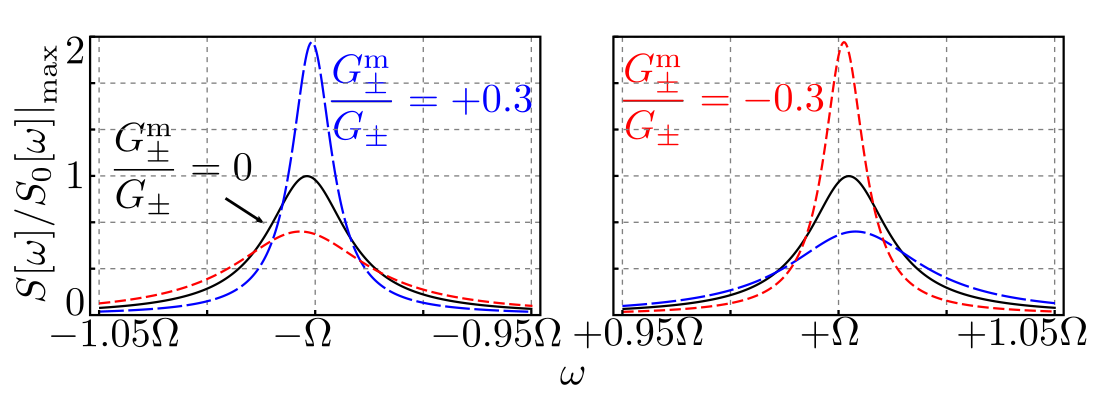
\includegraphics[width = 9 cm]{plots/plot_spectrum.png}
	\end{figure}	

	\begin{itemize}
		\item Centered around the detunings from the cavity resonance frequency
		\item Solid black curve without imperfections $G^{m}_{\pm}/G_{\pm} = 0$
		\item Imperfections on the effective couplings described by
	\end{itemize}

	\begin{figure}
		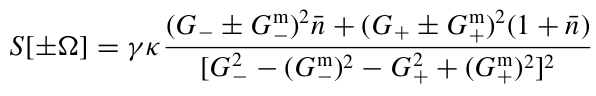
\includegraphics[width = 6.5 cm]{plots/spectrum_imperfections.png}
	\end{figure}

\end{frame}

% Experimental observability II
\begin{frame}
	
	\frametitle{Experimental observability}
	\framesubtitle{Output spectrum}	
	
	\begin{itemize}
		\item Experimental work realized in {\color{blue}"Stabilized entanglement of massive mechanical oscillators"}, Nature, 2018.
		\item Measure output spectrum and reconstruct quadratures to identify entanglement
	\end{itemize}

\end{frame}

% Conclusions
\begin{frame}

	\frametitle{Conclusions}
	
	\begin{enumerate}
		\item Configuring a three-mode optomechanical system such as the steady state includes highly pure and highly entangled two-mode squeezed state.
		\item Symmetry on the steady-state makes it attractive for implementation of  continuous-variable teleportation protocols
		\item Problem of unequal single-photon optomechanical couplings solved by using four-tone driving scheme
		\item Proposal implementable for existing technology
	\end{enumerate}
		
\end{frame}

% Conclusions
\begin{frame}
	
	\frametitle{Back up}
	\framesubtitle{Thermal occupation}
	
	\begin{enumerate}
		\item Occupation (photons) at $\omega_{c} \sim 10^{10} \textrm{Hz}$
		\begin{equation}
			\bar{n}_{\textrm{photons}} = \frac{1}{e^{\frac{\hbar \omega_{c}}{K_{B}T}} - 1} \simeq 0 \nonumber
		\end{equation}
		\item Occupation (phonons) $\longrightarrow \omega_{m} \sim 10 \; \textrm{KHz} - 1 \; \textrm{GHz}$
		\begin{equation}
			\bar{n}_{\textrm{photons}} = \frac{1}{e^{\hbar \omega_{c} / K_{B}T} - 1} \gg 1 \nonumber
		\end{equation}
	\end{enumerate}

\end{frame}

% Conclusions
\begin{frame}
	
	\frametitle{Back up}
	\framesubtitle{Counter rotating effects}
	
	\begin{enumerate}
		\item Occupation (photons) at $\omega_{c} \sim 10^{10} \textrm{Hz}$
		\begin{equation}
		\bar{n}_{\textrm{photons}} = \frac{1}{e^{\frac{\hbar \omega_{c}}{K_{B}T}} - 1} \simeq 0 \nonumber
		\end{equation}
		\item Occupation (phonons) $\longrightarrow \omega_{m} \sim 10 \; \textrm{KHz} - 1 \; \textrm{GHz}$
		\begin{equation}
		\bar{n}_{\textrm{photons}} = \frac{1}{e^{\hbar \omega_{c} / K_{B}T} - 1} \gg 1 \nonumber
		\end{equation}
	\end{enumerate}

\end{frame}

\end{document}